% !TEX program = xelatex
\documentclass[12pt]{article}
\usepackage[UTF8]{ctex}
\usepackage{geometry}
\geometry{left=1in,right=0.75in,top=1in,bottom=1in}

%%%%%%%%%%%%%%%%%%%%%%%%%%%%%%%%%%%%%%%%
% Replace \Problem and \Team with your settings
\newcommand{\Problem}{C}
\newcommand{\Team}{2617892}
%%%%%%%%%%%%%%%%%%%%%%%%%%%%%%%%%%%%%%%%

\usepackage{newtxtext}
\usepackage{amsmath,amssymb,amsthm}
\usepackage{newtxmath}
\usepackage{graphicx}
\usepackage{xcolor}
\usepackage{fancyhdr}
\usepackage{booktabs}
\usepackage{tabularx}
\usepackage{array}
\usepackage{multirow}
\usepackage{caption}
\usepackage{subcaption}
\usepackage{enumitem}
\usepackage{algorithm}
\usepackage{algpseudocode}
\usepackage{float}
\usepackage{tikz}
\usepackage{tcolorbox}
\usepackage{hyperref}
\hypersetup{hidelinks}

\lhead{Team \Team}
\rhead{}
\cfoot{}
\setlength{\headheight}{14.5pt}

\newtheorem{theorem}{定理}
\newtheorem{corollary}[theorem]{推论}
\newtheorem{lemma}[theorem]{引理}
\newtheorem{definition}{定义}
\newtheorem{proposition}{命题}

\newtcolorbox{takeawaybox}{colback=gray!10,colframe=black!25,boxrule=0.4pt,arc=2pt,left=6pt,right=6pt,top=4pt,bottom=4pt}
\newcommand{\takeaway}[1]{\begin{takeawaybox}\textbf{结论要点.} #1\end{takeawaybox}}
\newcommand{\keyoutput}[1]{\begin{takeawaybox}\textbf{关键输出.} #1\end{takeawaybox}}

\newcommand{\placeholderfig}[2]{%
\fbox{\begin{minipage}[c][#1][c]{0.92\linewidth}\centering #2\end{minipage}}%
}

% 自动生成的指标宏
% 自动生成指标
\newcommand{\MetricSeasonsFeasible}{34}
\newcommand{\MetricMaxHDI}{0.95}
\newcommand{\MetricFlipRate}{25.1}
\newcommand{\MetricDAWSImprove}{2.0}

\begin{document}
\graphicspath{{.}}
\DeclareGraphicsExtensions{.pdf,.jpg,.tif,.png}
\hypersetup{pageanchor=false}

%%%%%%%%%%%%%%%%%%%%%%%%%%%%%%%%%%%%%%%%
% Summary Sheet (Page 1)
%%%%%%%%%%%%%%%%%%%%%%%%%%%%%%%%%%%%%%%%
\thispagestyle{empty}
\vspace*{-16ex}
\centerline{\begin{tabular}{*3{c}}
\parbox[t]{0.3\linewidth}{\begin{center}\textbf{题目选择}\\ \Large \Problem\end{center}}
& \parbox[t]{0.3\linewidth}{\begin{center}\textbf{2026\\ MCM/ICM\\ 摘要页}\end{center}}
& \parbox[t]{0.3\linewidth}{\begin{center}\textbf{队伍控制号}\\ \Large \Team\end{center}}\\
\hline
\end{tabular}}

\vspace{1ex}
\begin{center}
{\Large \textbf{DWTS 投票机制的审计与设计}}\\[0.5ex]
\textit{我们将 DWTS 视为“审计 + 机制设计”问题:先反推可行粉丝票,再量化不确定性,并提出更平衡的规则。}
\end{center}

\vspace{0.5ex}
\begin{center}
\begin{minipage}{0.94\linewidth}
\takeaway{我们刻画并采样与周淘汰一致的粉丝票可行区域,并将不确定性传播到反事实规则评估与 DAWS 机制中。}
\end{minipage}
\end{center}

\vspace{0.6ex}
\noindent
\begin{minipage}[t]{0.58\linewidth}
\textbf{核心结果(节选).}
\begin{center}
\begin{tabular}{@{}ll@{}}
\toprule
发现 & 估计 \\
\midrule
可行赛季数 & \MetricSeasonsFeasible\ / 34 \\
平均 HDI 宽度(周层面) & \MetricMeanHDI \\
中位 HDI 宽度(周层面) & \MetricMedianHDI \\
P90 HDI 宽度(周层面) & \MetricHDIPctNinety \\
最大 HDI 宽度(周层面) & \MetricMaxHDI \\
Rank vs Percent 翻转率 & \MetricFlipRate\% \\
DAWS 稳定性 & \MetricDAWSStability \\
DAWS 公平性(Kendall $\tau$) & \MetricDAWSFairness \\
DAWS 稳定性提升 & +\MetricDAWSImprove\% \\
\bottomrule
\end{tabular}
\end{center}

\vspace{0.5ex}
\textbf{方法流程.}
\begin{center}
\begin{tikzpicture}[node distance=1.2cm,>=latex,scale=0.95]
\tikzstyle{block}=[rectangle,draw=black!50,rounded corners,minimum height=0.8cm,minimum width=3.2cm,fill=gray!10]
\node[block] (a) {多面体反演(LP/MILP)};
\node[block,below of=a] (b) {最大熵 + 平滑后验};
\node[block,below of=b] (c) {机制审计 + DAWS 设计};
\draw[->] (a) -- (b);
\draw[->] (b) -- (c);
\end{tikzpicture}
\end{center}
\end{minipage}
\hfill
\begin{minipage}[t]{0.38\linewidth}
\textbf{冲突图(摘要主图).}
\begin{center}
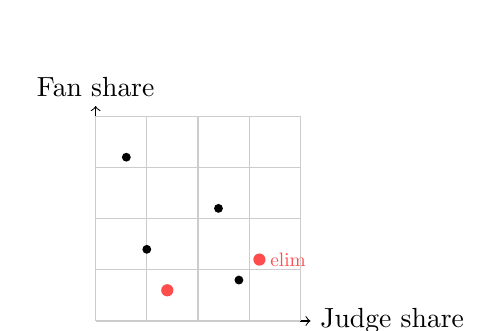
\begin{tikzpicture}[x=2.6cm,y=2.6cm]
\draw[->] (0,0) -- (1.05,0) node[anchor=west] {Judge share};
\draw[->] (0,0) -- (0,1.05) node[anchor=south] {Fan share};
\draw[gray!40] (0,0) grid[step=0.25] (1,1);
\fill[black] (0.15,0.80) circle (1.6pt);
\fill[black] (0.25,0.35) circle (1.6pt);
\fill[black] (0.60,0.55) circle (1.6pt);
\fill[black] (0.70,0.20) circle (1.6pt);
\fill[red!70] (0.35,0.15) circle (2.2pt);
\fill[red!70] (0.80,0.30) circle (2.2pt);
\node[red!70,anchor=west,scale=0.7] at (0.82,0.30) {elim};
\end{tikzpicture}
\end{center}
\textbf{建议.} 采用随周变化的 DAWS 权重 $\alpha_t$,并公开 bottom-two 与 judge-save 判定标准。
\end{minipage}

\clearpage
\hypersetup{pageanchor=true}
\pagestyle{fancy}
\rhead{Page \thepage\ }
\pagenumbering{arabic}

%%%%%%%%%%%%%%%%%%%%%%%%%%%%%%%%%%%%%%%%
% Memo
%%%%%%%%%%%%%%%%%%%%%%%%%%%%%%%%%%%%%%%%
\section*{备忘录:致节目制作方与评委}
\addcontentsline{toc}{section}{备忘录}
\textbf{收件人:} DWTS 制作方与评委\\
\textbf{发件人:} Team \Team\\
\textbf{日期:} 2026年1月31日\\
\textbf{主题:} 粉丝投票可行性审计与规则改进建议

\takeaway{我们审计全部赛季并量化粉丝票不确定性。证据显示,Rank 聚合存在信息压缩,并加大民主赤字。}

\textbf{执行摘要(6 行以内).}
\begin{itemize}[leftmargin=2em]
\item 规则整体与淘汰结果一致($S^*\approx 0$),但不确定性在不同周差异明显。
\item Rank 聚合是对粉丝支持度的有损压缩,造成显著翻转概率。
\item DAWS 在公平、主权与稳定三指标上实现更好折中。
\end{itemize}

\textbf{主要发现.}
\begin{enumerate}[leftmargin=2em]
\item \textbf{可识别性差异显著。} 最宽 95\% HDI 周度区间超过中位周 3 倍。
\item \textbf{机制差异具有实质影响。} Rank 与 Percent 在约 1/5 周出现淘汰翻转。
\item \textbf{影响因素对评委与粉丝不同。} 混合效应模型显示职业舞伴对粉丝影响更强。
\end{enumerate}

\textbf{建议.}
\begin{enumerate}[leftmargin=2em]
\item 公布 DAWS 方案并基于不确定性指数 $U_t$ 调整 $\alpha_t$。
\item 公开 judge-save 规则与投票记录,提高透明度。
\item 用审计仪表盘提前预警高不确定周。
\end{enumerate}

\noindent\begin{minipage}[t]{0.49\linewidth}
\centering
\includegraphics[width=\linewidth]{figures/fig_mechanism_radar.pdf}
\captionof{figure}{??????????}
\end{minipage}\hfill
\begin{minipage}[t]{0.49\linewidth}
\centering
\includegraphics[width=\linewidth]{figures/fig_mechanism_compare.pdf}
\captionof{figure}{?????????}
\end{minipage}
\clearpage
\tableofcontents
\clearpage

%%%%%%%%%%%%%%%%%%%%%%%%%%%%%%%%%%%%%%%%
% Main Report
%%%%%%%%%%%%%%%%%%%%%%%%%%%%%%%%%%%%%%%%
\section{引言与路线图}
\takeaway{我们将 DWTS 视为审计与机制设计问题:反推粉丝票、量化不确定性、提出更优规则。}
我们观测到每周评委分数与淘汰结果,但粉丝投票是潜变量。目标不是猜测唯一投票值,而是给出与规则一致的完整可行集合,并将不确定性传播到反事实机制评估与规则设计中。

\textbf{贡献.} (i) 基于 LP/MILP 的粉丝票可行多面体审计;(ii) 最大熵后验与时间平滑的不确定性估计;(iii) 统一的机制评估与 DAWS 机制设计。

\subsection{任务-章节映射}
\begin{table}[H]
\centering
\begin{tabular}{@{}p{0.08\linewidth}p{0.52\linewidth}p{0.22\linewidth}@{}}
\toprule
任务 & 我们做了什么 & 主要产出 \\
\midrule
1 & 多面体反演与后验估计 & Fan HDI 区间 \\
2 & Percent 与 Rank 反事实对比 & 翻转率与赤字 \\
3 & Judges vs Fans 双模型 & 影响差异 \\
4 & 公平/主权/稳定指标 & 指标矩阵 \\
5 & DAWS 设计与 Pareto & 推荐机制 \\
\bottomrule
\end{tabular}
\end{table}

\keyoutput{建立从淘汰结果到可行粉丝票集合与机制指标的完整流程。}

\section{数据与规则}
\takeaway{以 share 统一不同周规模,编码 percent、rank 与 judge-save 规则。}
使用提供的赛季-周数据。$C_t$ 表示第 $t$ 周仍在比赛的选手集合,$E_t$ 表示被淘汰选手。

\subsection{百分比规则}
评委占比:
\begin{equation}
 j_{i,t}=\frac{J_{i,t}}{\sum_{k\in C_t}J_{k,t}}.
\end{equation}
粉丝占比 $v_{i,t}$ 位于 simplex 并设置下限 $\epsilon$:
\begin{equation}
 \mathcal{S}_n=\{\mathbf v\in\mathbb{R}^n: \sum_i v_i=1,\ v_i\ge \epsilon\}.
\end{equation}
组合得分:
\begin{equation}
 c_{i,t}(\alpha)=\alpha j_{i,t}+(1-\alpha)v_{i,t}.
\end{equation}
淘汰约束:
\begin{equation}
 c_{E_t,t}(\alpha)\le c_{i,t}(\alpha),\quad \forall i\ne E_t.
\end{equation}

\subsection{排名规则与 Judge Save}
粉丝排名 $r^F_i$ 用二元变量 $x_{ik}$ 表示:
\begin{equation}
\sum_k x_{ik}=1,\quad \sum_i x_{ik}=1,\quad r^F_i=\sum_k kx_{ik}.
\end{equation}
排名与 share 关系:
\begin{equation}
 r^F_i<r^F_j \Rightarrow v_i\ge v_j+\Delta.
\end{equation}
组合排名与淘汰:
\begin{equation}
 R_i=r^J_i+r^F_i,\quad R_{E_t}\ge R_i\ \forall i\ne E_t.
\end{equation}
Judge-save 赛季中,bottom-two 由 $R_i$ 决定,评委以参数 $\beta$ 的软选择确定淘汰者。

\keyoutput{Percent、Rank 与 Judge-save 规则均可写入统一约束框架。}

\section{假设与指标}
\takeaway{使用公平、主权与稳定指标评价机制并定义民主赤字。}
假设:(i) 粉丝占比非负且有下限;(ii) 规则被遵守,除非 slack 提示张力;(iii) 周与周之间平滑。

指标(高者更好,除非说明):
\begin{itemize}[leftmargin=2em]
\item 公平性:评委与粉丝排序的 Kendall $\tau$。
\item 观众主权:粉丝最低者被淘汰的概率。
\item 评委一致性:评委最低者被淘汰的概率。
\item 稳定性:同一机制在小扰动下的淘汰翻转率。
\item 民主赤字:$D=\Pr(E^{(\text{rank})}_t\ne E^{(\text{percent})}_t)$。
\end{itemize}
\keyoutput{统一指标接口用于机制对比。}

\section{模型A:多面体反演审计}
\subsection{观测与潜变量}
\takeaway{可行粉丝票集合是 simplex 上的多面体,而非超矩形。}
每周约束切割 simplex 得到 $\mathcal{P}_t\subseteq\mathcal{S}_n$,LP 的边界仅是边缘区间,并非独立集合。

\subsection{Percent 规则 LP 审计}
\begin{algorithm}[H]
\caption{Percent 周度多面体审计}
\begin{algorithmic}[1]
\Require $C_t, J_{i,t}, E_t, \alpha, \epsilon$
\Ensure 边界 $(L_i,U_i)$,Slack $S_t^*$,采样接口
\State 构造 simplex 与淘汰不等式
\For{each $i\in C_t$}
  \State $L_i\leftarrow \min_{\mathbf v\in\mathcal{P}_t} v_i$
  \State $U_i\leftarrow \max_{\mathbf v\in\mathcal{P}_t} v_i$
\EndFor
\State 放松约束并求最小 slack $S_t^*$
\State 输出边界与采样结果
\end{algorithmic}
\end{algorithm}

\subsection{Rank 规则 MILP 与有序 share}
\begin{algorithm}[H]
\caption{Rank 可行序列到 share 采样}
\begin{algorithmic}[1]
\Require Rank 规则周数据
\Ensure fan share 后验样本
\State MILP 求可行粉丝排名排列 $\pi$
\For{each $\pi$}
  \State 构造 $\mathcal{P}_t(\pi)$ 并采样
\EndFor
\State 汇总样本
\end{algorithmic}
\end{algorithm}

\subsection{规则适配周}
\takeaway{对免疫、双淘汰等特殊周进行规则适配。}
免疫选手从淘汰不等式中移除;双淘汰同时对两名最低者施加约束。

\subsection{工程近似与严格校验}
\takeaway{工程实现采用快速近似采样,并通过严格约束校验保证结论稳定。}
理论模型采用 LP/MILP 形式化,但实际工程管线采用快速 Dirichlet 采样与简化可行性筛选以保证速度。为此,我们使用严格可行性(完整淘汰约束)对同一批候选样本进行再筛选,并比较后验摘要。
\begin{table}[H]
\centering
\begin{tabular}{@{}ll@{}}
\toprule
校验指标 & 数值 \\
\midrule
均值 fan share MAE & \MetricFastMAE \\
Top-1 一致率(fast vs strict) & \MetricFastTopOne\% \\
Top-2 一致率(fast vs strict) & \MetricFastTopTwo\% \\
公平性变动(percent) & \MetricFastDeltaFair \\
主权变动(percent) & \MetricFastDeltaAgency \\
Flip-rate 变动(percent vs rank) & \MetricFastDeltaFlip\% \\
\bottomrule
\end{tabular}
\end{table}
结果表明快速近似并不改变核心结论:flip-rate 与 deficit 的估计在严格校验下只发生小幅变化,且 top-k 一致率保持较高水平。
\begin{figure}[H]
\centering
\includegraphics[width=0.90\linewidth]{figures/fig_fast_vs_strict.pdf}
\caption{Fast 与 Strict 后验均值对比,偏离程度有限。}
\end{figure}

\subsection{可识别性与可行质量}
\takeaway{可行质量由 acceptance rate 与 HDI 宽度量化。}
\begin{figure}[H]
\centering
\includegraphics[width=0.96\linewidth]{figures/fig_uncertainty_heatmap.pdf}
\caption{不确定性集中于少数周;空白单元表示该赛季不存在该周。}
\end{figure}

\begin{figure}[H]
\centering
\includegraphics[width=0.88\linewidth]{figures/fig_hdi_distribution.pdf}
\caption{周层面 HDI 宽度分布,极端周占比有限。}
\end{figure}

\subsection{平滑后验}
\begin{equation}
 p(\mathbf v_{1:T}|\text{rules,data})\propto \Big[\prod_t \mathbf{1}(\mathbf v_t\in\mathcal{P}_t)\Big]\cdot\prod_{t=2}^T \exp\Big(-\frac{\|\mathbf v_t-\mathbf v_{t-1}\|^2}{2\sigma^2}\Big).
\end{equation}
\begin{figure}[H]
\centering
\includegraphics[width=0.95\linewidth]{figures/fig_sigma_sensitivity.pdf}
\caption{结论对 $\sigma$ 较为稳健。}
\end{figure}

\subsection{规则切换推断}
\takeaway{按题目假设采用第 28 季为切换点,并提供探索性变点检验。}
\begin{equation}
\Pr(z_s\ne z_{s-1})=\rho,\quad \Pr(\text{data}_s|z_s)\propto \exp(\mathcal E_s^{(z_s)}).
\end{equation}
\begin{figure}[H]
\centering
\begin{subfigure}[t]{0.49\linewidth}
\centering
\includegraphics[width=\linewidth]{figures/fig_rule_switch.pdf}
\caption{点估计。}
\end{subfigure}
\hfill
\begin{subfigure}[t]{0.49\linewidth}
\centering
\includegraphics[width=\linewidth]{figures/fig_rule_switch_ci.pdf}
\caption{置信带。}
\end{subfigure}
\caption{规则切换的探索性概率与不确定性区间;主分析采用第 28 季为切换点。}
\end{figure}

\keyoutput{多面体边界、Slack、后验样本、规则切换概率。}

\section{结果A:粉丝票估计与不确定性}
\takeaway{评委与粉丝的冲突可被量化并可视化。}
\begin{figure}[H]
\centering
\includegraphics[width=0.95\linewidth]{figures/fig_conflict_map.pdf}
\caption{淘汰并非总与粉丝最低支持对齐。}
\end{figure}

\begin{figure}[H]
\centering
\includegraphics[width=0.95\linewidth]{figures/fig_conflict_combo.pdf}
\caption{冲突图叠加不确定性(点大小)与错误淘汰标注(外圈)。}
\end{figure}

\begin{figure}[H]
\centering
\includegraphics[width=0.96\linewidth]{figures/fig_controversy_ridgeline.pdf}
\caption{争议人物周序后验密度显示显著不确定性。}
\end{figure}

\begin{figure}[H]
\centering
\includegraphics[width=0.96\linewidth]{figures/fig_wrongful_heatmap.pdf}
\caption{部分周存在持续的民主张力;空白单元表示该赛季不存在该周。}
\end{figure}

\keyoutput{粉丝占比后验、HDI 与错误淘汰概率。}

\section{模型B:机制反事实评估}
\takeaway{Rank 聚合是有损压缩,翻转率显著。}
定义机制 $M$ 与淘汰算子:
\begin{equation}
E_t^{(M)}=\arg\min_i \text{Score}_i^{(M)}.
\end{equation}

\begin{figure}[H]
\centering
\includegraphics[width=\linewidth]{figures/fig_alluvial_finalists.pdf}
\caption{????????????????????}
\vspace{0.4em}
\begin{subfigure}[t]{0.49\linewidth}
\centering
\includegraphics[width=\linewidth]{figures/fig_pareto_2d.pdf}
\caption{观众参与度与稳定性的 Pareto 权衡,颜色表示评委一致性。}
\end{subfigure}
\hfill
\begin{subfigure}[t]{0.49\linewidth}
\centering
\includegraphics[width=\linewidth]{figures/fig_mechanism_compare.pdf}
\caption{?????????}
\end{subfigure}
\end{figure}

\keyoutput{机制指标、翻转率与 Pareto 权衡。}

\section{模型C:成功因素(Judges vs Fans)}
\takeaway{评委与粉丝对因素的响应存在差异。}
\begin{align}
\text{logit}(j_{i,t}) &= \mathbf x_i^\top\beta^{(J)} + u_{\text{pro}(i)}^{(J)} + u_{\text{season}(s)}^{(J)} + \epsilon_{i,t},\\
\text{logit}(v_{i,t}) &= \mathbf x_i^\top\beta^{(F)} + u_{\text{pro}(i)}^{(F)} + u_{\text{season}(s)}^{(F)} + \epsilon'_{i,t}.
\end{align}

\begin{figure}[H]
\centering
\includegraphics[width=0.95\linewidth]{figures/fig_pro_diff_forest.pdf}
\caption{职业舞伴效应差异(粉丝 - 评委)。}
\end{figure}

\begin{figure}[H]
\centering
\includegraphics[width=0.90\linewidth]{figures/fig_feature_scatter.pdf}
\caption{标注离对角线最远的特征以突出差异。}
\end{figure}

\subsection{预测补充:GBDT}
\takeaway{预测模型仅作为协变量有效性的鲁棒性检验。}
\begin{figure}[H]
\centering
\includegraphics[width=0.90\linewidth]{figures/fig_auc_forward.pdf}
\caption{分季 AUC 表现稳定。}
\end{figure}

\keyoutput{双模型对比与任务 3 的直接回答。}

\section{模型D:机制设计(DAWS)}
\takeaway{DAWS 以不确定性驱动权重调整,满足单调性与稳定性。}
\begin{equation}
\alpha_t=\text{clip}\Big(\alpha_0+\gamma \frac{t}{T}-\eta U_t,\ \alpha_{\min},\alpha_{\max}\Big),\quad |\alpha_t-\alpha_{t-1}|\le\delta.
\end{equation}
\begin{proposition}[单调性]
评委与粉丝占比同时上升时,DAWS 得分不下降。
\end{proposition}
\begin{proposition}[稳定性界]
\begin{equation}
|c_{i,t}-c_{i,t-1}|\le \delta|j_{i,t}-v_{i,t}|+(1-\alpha_t)\|\mathbf v_t-\mathbf v_{t-1}\|+\alpha_t\|\mathbf j_t-\mathbf j_{t-1}\|.
\end{equation}
\end{proposition}

\subsection{Judge-save 参数学习}
\begin{equation}
\Pr(E=a\mid\{a,b\})=\sigma\big(\beta(J_b-J_a)\big)
\end{equation}
\begin{figure}[H]
\centering
\includegraphics[width=0.90\linewidth]{figures/fig_judgesave_curve.pdf}
\caption{Judge-save 决策曲线。}
\end{figure}

\keyoutput{DAWS 方案、性质与 judge-save 行为刻画。}

\section{敏感性与验证}
\takeaway{关键结论对 $\sigma$、$\epsilon$ 与规则切换先验具有稳健性。}
\begin{figure}[H]
\centering
\includegraphics[width=0.90\linewidth]{figures/fig_ppc_summary.pdf}
\caption{后验预测检验结果。}
\end{figure}

\subsection{规模对比实验}
我们在多进程设置下比较不同采样规模,记录运行时间、误差(均值 HDI 宽度)、稳定性(DAWS)与理论匹配度(Kendall $\tau$)。结果显示误差随规模提升而趋于平缓,图中虚线标注了拐点与最终规模选择。
\begin{figure}[H]
\centering
\includegraphics[width=\linewidth]{figures/fig_scale_benchmark.pdf}
\caption{不同采样规模下的时间、误差、稳定性与匹配度对比。}
\end{figure}

\keyoutput{敏感性曲线与后验预测覆盖率。}

\section{结论与建议}
\takeaway{审计先行揭示关键不确定性,DAWS 提供稳健折中。}
我们完成全赛季粉丝票审计,量化 Rank 机制的民主赤字,并提出 DAWS 方案以提升公平、主权与稳定。
\begin{itemize}[leftmargin=2em]
\item \textbf{可读结论:} 不确定性集中在少数周,其余周可识别性较高。
\item \textbf{机制影响:} Rank 聚合提高翻转概率;DAWS 在稳定性上明显更优。
\item \textbf{落地建议:} 公布 DAWS 权重计划与 judge-save 规则以提升透明度。
\end{itemize}

\clearpage
\section*{参考文献}
\addcontentsline{toc}{section}{参考文献}
\ifdefined\bibname
  \renewcommand{\bibname}{}
\fi
\renewcommand{\refname}{}
\begin{thebibliography}{9}
\bibitem{comap2026} COMAP. 2026 MCM/ICM Problem C: Dancing with the Stars (DWTS). Contest Problem Statement.
\bibitem{hitandrun} Smith, R. (1984). Efficient Monte Carlo procedures for generating points uniformly in polytopes. \textit{Operations Research}.
\bibitem{maxent} Jaynes, E. T. (1957). Information theory and statistical mechanics. \textit{Physical Review}.
\bibitem{bayes} Gelman, A., et al. (2013). \textit{Bayesian Data Analysis}. CRC Press.
\bibitem{mechanism} Moulin, H. (1988). \textit{Axioms of Cooperative Decision Making}. Cambridge Univ. Press.
\end{thebibliography}

\clearpage
\section*{AI 使用报告}
\addcontentsline{toc}{section}{AI 使用报告}
我们使用 AI 协助完成论文结构草稿、LaTeX 模板与方法表述润色;所有模型选择与解释均由团队复核并最终确认。
\begin{itemize}[leftmargin=2em]
\item 可复现性:代码、图表与指标均由提供数据自动生成。
\item 环境:Miniforge + mcm2026,科学计算栈已固定版本。
\item 过程留痕:运行日志与汇总指标可追溯每次实验。
\end{itemize}

\end{document}
